
\documentclass[a4paper,11pt]{article}
\usepackage[a4paper, margin=8em]{geometry}

% usa i pacchetti per la scrittura in italiano
\usepackage[french,italian]{babel}
\usepackage[T1]{fontenc}
\usepackage[utf8]{inputenc}
\frenchspacing 

% usa i pacchetti per la formattazione matematica
\usepackage{amsmath, amssymb, amsthm, amsfonts}

% usa altri pacchetti
\usepackage{gensymb}
\usepackage{hyperref}
\usepackage{standalone}

% imposta il titolo
\title{Appunti Elettronica Digitale}
\author{Luca Seggiani}
\date{2026}

% imposta lo stile
% usa helvetica
\usepackage[scaled]{helvet}
% usa palatino
\usepackage{palatino}
% usa un font monospazio guardabile
\usepackage{lmodern}

\renewcommand{\rmdefault}{ppl}
\renewcommand{\sfdefault}{phv}
\renewcommand{\ttdefault}{lmtt}

% disponi il titolo
\makeatletter
\renewcommand{\maketitle} {
	\begin{center} 
		\begin{minipage}[t]{.8\textwidth}
			\textsf{\huge\bfseries \@title} 
		\end{minipage}%
		\begin{minipage}[t]{.2\textwidth}
			\raggedleft \vspace{-1.65em}
			\textsf{\small \@author} \vfill
			\textsf{\small \@date}
		\end{minipage}
		\par
	\end{center}

	\thispagestyle{empty}
	\pagestyle{fancy}
}
\makeatother

% disponi teoremi
\usepackage{tcolorbox}
\newtcolorbox[auto counter, number within=section]{theorem}[2][]{%
	colback=blue!10, 
	colframe=blue!40!black, 
	sharp corners=northwest,
	fonttitle=\sffamily\bfseries, 
	title=~\thetcbcounter: #2, 
	#1
}

% disponi definizioni
\newtcolorbox[auto counter, number within=section]{definition}[2][]{%
	colback=red!10,
	colframe=red!40!black,
	sharp corners=northwest,
	fonttitle=\sffamily\bfseries,
	title=~\thetcbcounter: #2,
	#1
}

% U.D.M
\newcommand{\amp}{\ensuremath{\mathrm{A}}}
\newcommand{\volt}{\ensuremath{\mathrm{V}}}
\newcommand{\meter}{\ensuremath{\mathrm{m}}}
\newcommand{\second}{\ensuremath{\mathrm{s}}}
\newcommand{\farad}{\ensuremath{\mathrm{F}}}
\newcommand{\henry}{\ensuremath{\mathrm{H}}}
\newcommand{\siemens}{\ensuremath{\mathrm{S}}}

% circuiti
\usepackage{circuitikz}
\usetikzlibrary{babel}

% disegni
\usepackage{pgfplots}
\pgfplotsset{width=10cm,compat=1.9}

% disponi codice
\usepackage{listings}
\usepackage[table]{xcolor}

\definecolor{codegreen}{rgb}{0,0.6,0}
\definecolor{codegray}{rgb}{0.5,0.5,0.5}
\definecolor{codepurple}{rgb}{0.58,0,0.82}
\definecolor{backcolour}{rgb}{0.95,0.95,0.92}

\lstdefinestyle{codestyle}{
		backgroundcolor=\color{black!5}, 
		commentstyle=\color{codegreen},
		keywordstyle=\bfseries\color{magenta},
		numberstyle=\sffamily\tiny\color{black!60},
		stringstyle=\color{green!50!black},
		basicstyle=\ttfamily\footnotesize,
		breakatwhitespace=false,         
		breaklines=true,                 
		captionpos=b,                    
		keepspaces=true,                 
		numbers=left,                    
		numbersep=5pt,                  
		showspaces=false,                
		showstringspaces=false,
		showtabs=false,                  
		tabsize=2
}

\lstdefinestyle{shellstyle}{
		backgroundcolor=\color{black!5}, 
		basicstyle=\ttfamily\footnotesize\color{black}, 
		commentstyle=\color{black}, 
		keywordstyle=\color{black},
		numberstyle=\color{black!5},
		stringstyle=\color{black}, 
		showspaces=false,
		showstringspaces=false, 
		showtabs=false, 
		tabsize=2, 
		numbers=none, 
		breaklines=true
}

\lstdefinelanguage{javascript}{
	keywords={typeof, new, true, false, catch, function, return, null, catch, switch, var, if, in, while, do, else, case, break},
	keywordstyle=\color{blue}\bfseries,
	ndkeywords={class, export, boolean, throw, implements, import, this},
	ndkeywordstyle=\color{darkgray}\bfseries,
	identifierstyle=\color{black},
	sensitive=false,
	comment=[l]{//},
	morecomment=[s]{/*}{*/},
	commentstyle=\color{purple}\ttfamily,
	stringstyle=\color{red}\ttfamily,
	morestring=[b]',
	morestring=[b]"
}

% disponi sezioni
\usepackage{titlesec}

\titleformat{\section}
	{\sffamily\Large\bfseries} 
	{\thesection}{1em}{} 
\titleformat{\subsection}
	{\sffamily\large\bfseries}   
	{\thesubsection}{1em}{} 
\titleformat{\subsubsection}
	{\sffamily\normalsize\bfseries} 
	{\thesubsubsection}{1em}{}

% disponi alberi
\usepackage{forest}

\forestset{
	rectstyle/.style={
		for tree={rectangle,draw,font=\large\sffamily}
	},
	roundstyle/.style={
		for tree={circle,draw,font=\large}
	}
}

% disponi algoritmi
\usepackage{algorithm}
\usepackage{algorithmic}
\makeatletter
\renewcommand{\ALG@name}{Algoritmo}
\makeatother

% disponi numeri di pagina
\usepackage{fancyhdr}
\fancyhf{} 
\fancyfoot[L]{\sffamily{\thepage}}

\makeatletter
\fancyhead[L]{\raisebox{1ex}[0pt][0pt]{\sffamily{\@title \ \@date}}} 
\fancyhead[R]{\raisebox{1ex}[0pt][0pt]{\sffamily{\@author}}}
\makeatother

\begin{document}
% sezione (data)
\section{Lezione del 05-05-26}

% stili pagina
\thispagestyle{empty}
\pagestyle{fancy}

% testo
Nella scorsa lezione avevamo introdotto le porte logiche digitali, e alcune caratteristiche come le temporizzazioni di risposta, l'uso di potenza e il fan-in/fan-out.

\subsection{Famiglie logiche}
Veniamo adesso a trattare le \textbf{famiglie logiche}, cioè categorie di componenti elettronici digitali basati sulla stessa tecnologia, e quindi fra di loro interoperabili. Per interconnettere fra di loro porte appartenenti a più famiglie, avremo chiaramente bisogno di reti di \textit{interfaccia}.

\subsubsection{Tecnologia CMOS}
La tecnologia per l'implementazione di famiglie logiche più importante che vediamo è quella \textbf{CMOS} (\textit{Complementary Metal Oxide Semiconductor}), che permette di utilizzare sullo stesso substrato di silicio sia MOSFTET di tipo PMOS che di tipo NMOS, dalle caratteristiche elettriche simili.

Distinguiamo più famiglie della tecnologia CMOS:
\begin{itemize}
	\item \textit{CMOS complementare}, che vedremo nel dettaglio;
	\item \textit{Logica pass-transistor}, che vedremo seppur in meno dettaglio;
	\item \textit{Logica dinamica} e \textit{pseudo NMOS}, che non vedremo.
\end{itemize}

Notiamo che esistono anche famiglie logiche basate sulla tecnologia bipolare, fra cui ad esempio la \textbf{TTL} (\textit{Transistor-Transistor Logic}) o la \textbf{RTL} (\textit{Resistor-Transistor Logic}), di cui era ad esempio parte l'inverter a carico resistivo. Non vediamo però queste famiglie in quanto sono state in larga parte soppiantate dal CMOS.

\subsubsection{Inverter}
Iniziamo la trattazione dei componenti digitali vedendo il più semplice, cioè l'\textbf{inverter}. Di base, l'inverter sarà un circuito disposto come segue:
\begin{center}
\begin{tikzpicture}[transform shape]
	% Paths, nodes and wires:
	\draw (0, 3) to[american resistor, l=$R$] (0, 1);
	\node[vcc] at (0, 3){};
	\draw (0, 1) to[switch] (0, -0);
	\draw[-stealth] (0, 1) -- (2, 1);
	\node[ground] at (0, -0){};
	\draw (-2, 0.5) -- (-0.25, 0.5);
	\draw[dash pattern={on 0.4pt off 1.6pt}] (-0.25, 0.5) -- (0, 0.75);
	\node[shape=rectangle, minimum width=0.465cm, minimum height=0.465cm] at (-2.5, 0.5){} node[anchor=center, align=center, text width=0.077cm, inner sep=6pt] at (-2.5, 0.5){$V_{in}$};
	\node[shape=rectangle, minimum width=0.465cm, minimum height=0.465cm] at (2.4, 1){} node[anchor=center, align=center, text width=0.077cm, inner sep=6pt] at (2.1, 1){$V_{out}$};
\end{tikzpicture}
\end{center}

Dove averemo un qualche tipo di interruttore comandato in tensione, che permetterà di far passare alternativamente corrente fra $V_{cc}$ e ground. Campionando $V_{out}$ prima di $R$, si ottiene effettivamente il comportamento di un inverter, dove a $V_{in}$ positiva corrisponde $V_{out}$ nulla.

Chiaramente dovrà valere, rispetto al comportamento dell'interruttore:
$$
\begin{cases}
	V_{in} = 0 \, \mathrm{V} \ \rightarrow \ \text{interruttore aperto} \\
	V_{out} = V_{cc}
\end{cases}, \quad
\begin{cases}
	V_{in} = V_{cc} \ \rightarrow \ \text{interruttore chiuso} \\
	V_{out} = 0 \, \mathrm{V} 
\end{cases}
$$

Il problema sarà quindi come implementare l'interruttore pilotato in tensione. A seconda della famiglia logica usata, la risposta più semplice sarà un transistore (BJT o MOSFET).

Infatti, abbiamo già visto l'inverter a carico resistivo NPN, e possiamo dire che anche i primi inverter realizzati in tecnologia MOSFET avevano la stessa topologia (cambiando solo la tipologia del transistor, e per le caratteristiche del MOSFET, trascurando la resistenza al segnale):
\begin{center}
\begin{tikzpicture}[transform shape]
	% Paths, nodes and wires:
	\draw (0, 3) to[american resistor] (0, 1);
	\node[vcc] at (0, 3){};
	\draw[-stealth] (0, 1) -- (2, 1);
	\node[ground] at (0, -0){};
	\node[shape=rectangle, minimum width=0.465cm, minimum height=0.465cm] at (-3, 0.5){} node[anchor=center, align=center, text width=0.077cm, inner sep=6pt] at (-3, 0.5){$V_{in}$};
	\node[shape=rectangle, minimum width=0.465cm, minimum height=0.465cm] at (2.5, 1){} node[anchor=center, align=center, text width=0.077cm, inner sep=6pt] at (2.1, 1){$V_{out}$};
	\node[npn] at (0, 0.48){};
	\draw (-2, 0.5) to[american resistor] (-0.84, 0.48);
	\draw (-2, 0.5) |- (-2.5, 0.5);
	\draw (7, 3) to[american resistor] (7, 1);
	\node[vcc] at (7, 3){};
	\draw[-stealth] (7, 1) -- (9, 1);
	\node[ground] at (7, -0){};
	\node[shape=rectangle, minimum width=0.465cm, minimum height=0.465cm] at (4, 0.5){} node[anchor=center, align=center, text width=0.077cm, inner sep=6pt] at (4, 0.5){$V_{in}$};
	\node[shape=rectangle, minimum width=0.465cm, minimum height=0.465cm] at (9.5, 1){} node[anchor=center, align=center, text width=0.077cm, inner sep=6pt] at (9.1, 1){$V_{out}$};
	\draw (6.02, 0.52) |- (4.52, 0.52);
	\node[nmos] at (7, 0.52){};
\end{tikzpicture}
\end{center}

Ricordiamo brevemente le caratteristiche dei transistori BJT e MOSFET, abbiamo che la retta di carico sul nostro circuito sarà data da  $\frac{V_{cc}}{R}$ dove $R$ è la resistenza al $V_{cc}$. Questa andrà ad intercettare una curva di risposta del transistor, che sarà modulata in valore massimo dalla corrente (per il BJT) o la tensione (per il MOSFET) alla base (cioè la nostra $V_{in})$. Aumentando la tensione all'ingresso, quindi, in entrambi i casi si permette la conduzione di corrente da $V_{cc}$ a ground, cioè si chiude il nostro "interruttore pilotato in tensione", che è esattamente ciò che volevamo fare.

In particolare, ricordiamo che nel caso BJT l'interruttore può considerarsi chiuso quando $V_{in} < V_\gamma$ e il transistor è in interdizione, mentre si considera come totalmente aperto quando $V_{in} = V_{cc}$, notando la piccola perdita data dalla tensione di saturazione $V_{CE,sat}$.

\par\smallskip

Una problematica data dall'implementazione degli inverter in questo modo è che quando la tensione $V_{in}$ è a $V_{cc}$, cioè l'interruttore è chiuso e l'inverter ha uscita bassa, c'è conduzione di corrente da $V_{cc}$ a $R$. Questo porta a dissipazione di potenza sulla resistenza $R$, proporzionale a $V_{cc}^2$. Tale situazione è inaccettabile nel caso in cui il risparmio energetico è una priorità.

Propioniamo allora una soluzione alternativa basata su 2 interruttori anziché uno:
\begin{center}
\begin{tikzpicture}[transform shape]
	% Paths, nodes and wires:
	\draw (0, 2.005) to[switch, l=$1$] (0, 0.005);
	\draw (0, 0.005) to[switch, l=$2$] (0, -1.995);
	\draw[-stealth] (0, -0) -- (2, -0);
	\node[vcc] at (0, 2.005){};
	\node[ground] at (0, -2){};
	\draw (-3, -0) -- (-1, -0);
	\draw[dash pattern={on 0.4pt off 1.6pt}] (-0.25, 1) |- (-1, 1) -| (-1, -1) -- (-0.25, -1);
	\node[shape=rectangle, minimum width=0.465cm, minimum height=0.465cm] at (-3.5, -0){} node[anchor=center, align=center, text width=0.077cm, inner sep=6pt] at (-3.6, -0){$V_{in}$};
	\node[shape=rectangle, minimum width=0.465cm, minimum height=0.465cm] at (2.25, -0){} node[anchor=center, align=center, text width=0.077cm, inner sep=6pt] at (2.25, -0){$V_{out}$};
\end{tikzpicture}
\end{center}

In questo caso attivando selettivamente solo uno dei 2 interruttori si potrà collegare la $V_{out}$ direttamente a $V_{cc}$ o a massa, quindi implementando l'inverter senza conduzione di corrente. La caratteristica che richiediamo all'interrutter sarà:
$$
\begin{cases}
	V_{in} = 0 \, \mathrm V \ \rightarrow \ \text{1 aperto, 2 chiuso} \\
	V_{out} = V_{cc}
\end{cases}, \quad
\begin{cases}
	V_{in} = V_{cc} \, \mathrm V \ \rightarrow \ \text{1 chiuso, 2 aperto} \\
	V_{out} = 0 \, \mathrm{V} 
\end{cases}
$$

Resta il problema di come implementare i 2 interruttori che rispettano questa caratteristica. Ricordiamo allora che i MOSFET PMOS e NMOS sono componenti effettivamente duali, cioè con caratteristiche identiche ma inverse. Questo ci permette di realizzare il seguente circuito:
\begin{center}
\begin{tikzpicture}[transform shape]
	% Paths, nodes and wires:
	\draw[-stealth] (0, -0) -- (2, -0);
	\node[vcc] at (0, 2.005){};
	\node[ground] at (0, -2){};
	\draw (-3, -0) -- (-1, -0);
	\node[shape=rectangle, minimum width=0.465cm, minimum height=0.465cm] at (-3.5, -0){} node[anchor=center, align=center, text width=0.077cm, inner sep=6pt] at (-3.6, -0){$V_{in}$};
	\node[shape=rectangle, minimum width=0.465cm, minimum height=0.465cm] at (2.25, -0){} node[anchor=center, align=center, text width=0.077cm, inner sep=6pt] at (2.25, -0){$V_{out}$};
	\node[nmos] at (0, -1){};
	\node[nmos] at (0.002, -1.004){};
	\node[pmos] at (0, 0.98){};
	\draw (-0.98, 0.98) |- (-0.978, -1.004);
	\draw (0, 1.75) -| (0, 2);
	\draw (0, 0.21) -| (0, -0.23);
	\draw (0, -1.77) -| (0, -2);
\end{tikzpicture}
\end{center}

Dove abbiamo un PMOS per interruttore 1, e un NMOS per interruttore 2. Prerogativa di questa configurazione sarà che le caratteristiche dei 2 MOSFET siano il più simmetriche possibile. 

\subsection{CMOS complementare}
La tecnologia che abbiamo appena visto per l'inverter è quella che sta alla base della famiglia \textit{CMOS complementare}.

\begin{center}
\begin{tikzpicture}[transform shape]
	% Paths, nodes and wires:
	\draw (-5, -0) -- (-3, -0);
	\draw (-1, 1.5) |- (-3, 1.5) -- (-3, -1.5) -- (-1, -1.5);
	\draw (0, -0) -- (3, -0);
	\node[shape=rectangle, draw, line width=1pt, minimum width=1.965cm, minimum height=1.965cm] at (0, 1.5){} node[anchor=center, align=center, text width=1.577cm, inner sep=6pt] at (0, 1.5){\scriptsize PULL-UP\\network};
	\node[shape=rectangle, draw, line width=1pt, minimum width=1.965cm, minimum height=1.965cm] at (0, -1.5){} node[anchor=center, align=center, text width=1.577cm, inner sep=6pt] at (0, -1.5){\scriptsize PULL-DOWN\\network};
	\draw (0, 0.5) -| (0, -0.5);
	\node[shape=rectangle, minimum width=0.465cm, minimum height=0.465cm] at (-5.5, -0){} node[anchor=center, align=center, text width=0.077cm, inner sep=6pt] at (-5.5, -0){$V_{in}$};
	\node[shape=rectangle, minimum width=0.465cm, minimum height=0.465cm] at (3.25, -0){} node[anchor=center, align=center, text width=0.077cm, inner sep=6pt] at (3.25, -0){$V_{out}$};
	\node[vcc] at (0, 2.5){};
	\node[ground] at (0, -2.5){};
\end{tikzpicture}
\end{center}

Solitamente l'approccio adottato nella CMOS complementare è una generalizzazione dell'inverter, dove si creano due reti duali, una di PMOS e una di NMOS:
\begin{itemize}
	\item La rete di PMOS viene detta \textit{pull-up network} ed è collegata al $V_{cc}$;
	\item La rete di NMOS viene detta \textit{pull-down network} ed è collegata a massa.
\end{itemize}
Le due reti vengono messe in serie, e fra di loro si preleva la tensione di uscita $V_{out}$. Gli $N$ ingressi delle reti pull-up e pull-down vengono invece messi a nodo comune e collegati agli $N$ ingressi $V_{in}$ di tutto il componente. L'obiettivo è di ottenere un comportamento che è simmetrico per la rete di pull-up e pull-down, che a stessi ingressi rispettivamente:
\begin{itemize}
	\item O attaccano a $V_{cc}$ staccando da massa (conduce la rete pull-up di PMOS);
	\item O attaccano a massa staccando da $V_{cc}$ (conduce la rete pull-down di NMOS).
\end{itemize}

Conseguenza naturale di questa tecnologia è che abbiamo bisogno del doppio dei transistor per realizzare una data rete (infatti questi verranno a coppie PMOS-NMOS).

\subsubsection{Analisi di circuiti in CMOS complementare}

Iniziamo a vedere l'analisi dei circuiti digitali a tecnologia CMOS complementare, partendo dall'esempio dell'inverter. Ciò che vorremo ricavare è la funzione di trasferimento, o meglio la \textbf{VTC} (\textit{Voltage Transfer Characteristic}) del circuito.

Chiamiamo quindi $i_{DN}$ la corrente fra drain e source del transistore NMOS, e $i_{DP}$ la corrente fra drain e source del transistore PMOS (notando che drain e source sono in posizioni invertite, cioè i drain stanno dalla parte della $V_{out}$ e i source a $V_{cc}$ e massa rispettivamente). In generale, se le caratteristiche delle reti di pull-down e pull-up sono simmetriche, dovrà valere:
$$
i_{DN} = - i_{DP}
$$

A partire dalla $i_{DN}$ definiamo la $V_{DSN}$, cioè la differenza di potenziale fra drain e source dell'NMOS, e la $V_{GSN}$, cioè la differenza di potenziale fra gate e source dell'NMOS. Visto che il source del NMOS è a massa, abbiamo che valgono le corrispondenze:
$$
V_{DSN} = V_{out}, \quad V_{GSN} = V_{in}
$$
Ricordando quanto detto sul grafico delle risposte in corrente dei MOSFET (ad esempio in 16.0.4), vediamo allora che il grafico dell'NMOS risulta più comodo, in quanto rappresenta direttamente la risposta della $V_{out}$ in funzione della $V_{in}$:
\begin{center}
	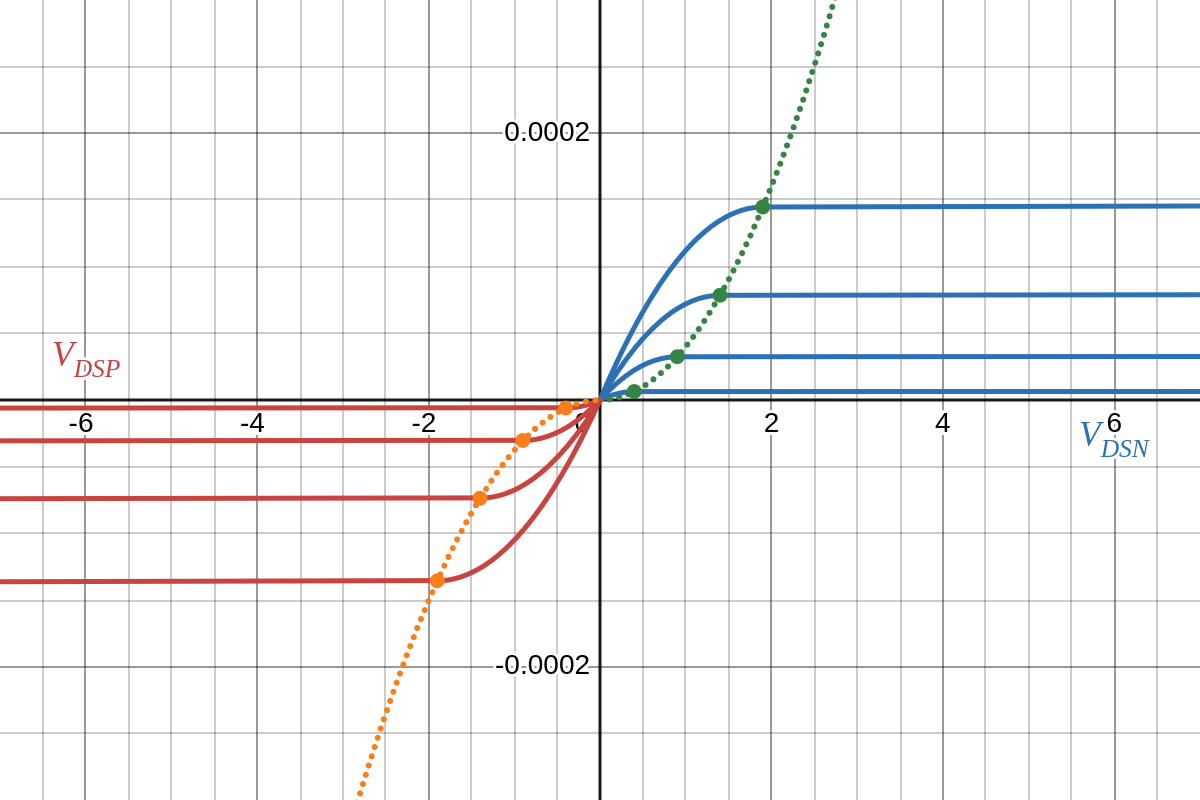
\includegraphics[scale=0.28]{../figures/cmos_char.png}
\end{center}

Vorremo quindi riportare la risposta del PMOS al primo quadrante (dove sta la risposta dell'NMOS). Facciamo ciò in 2 passaggi:
\begin{enumerate}
\item \textit{Ribaltamento} della risposta del PMOS sul secondo quadrante, che può essere fatto come:
$$
i_{DSP} = -i_{SDP} = -i_{DSN}
$$
\item \textit{Scostamento} della risposta del PMOS in maniera da riportarla sul primo quadrante, che può essere fatto come:
$$
\begin{cases}
V_{DSN} = V_{DSP} + V_{DD} \\
V_{DSP} = V_{DSN} - V_{DD} % qui non torna, sul gate ?
\end{cases}
$$
\end{enumerate}

Sul grafico questo ha il seguente aspetto, dove riportiamo in blu la $i_{DN}$ e in rosso la $-i_{DP}$.
\begin{center}
	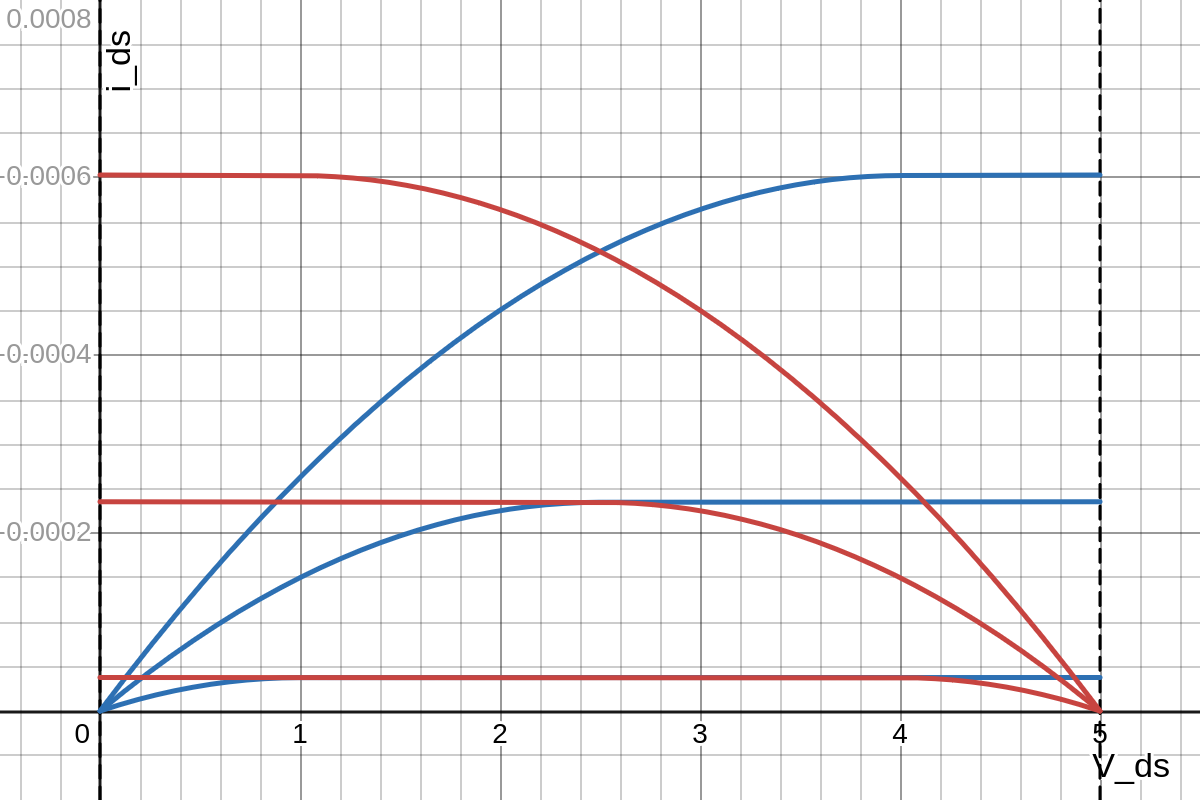
\includegraphics[scale=0.28]{../figures/cmos_ribalt.png}
\end{center}
La soluzione del circuito sarà chiaramente data dalle intersezione di una coppia di curve (una per il PMOS e una per l'NMOS).

Nel caso particolare dell'inverter, abbiamo che la variabile di controllo sull'NMOS è la $V_{in}$, mentre sul PMOS è:
$$
V_{GSP} = V_{GSN} - V_{CC} = V_{in} - V_{CC}
$$
Tracciando il grafico sopra fissando un valore di $V_{in}$, ad esempio $1 \, \mathrm{V}$ su una $V_{CC}$ di $5 \, \mathrm{V}$, otteniamo:
\begin{center}
	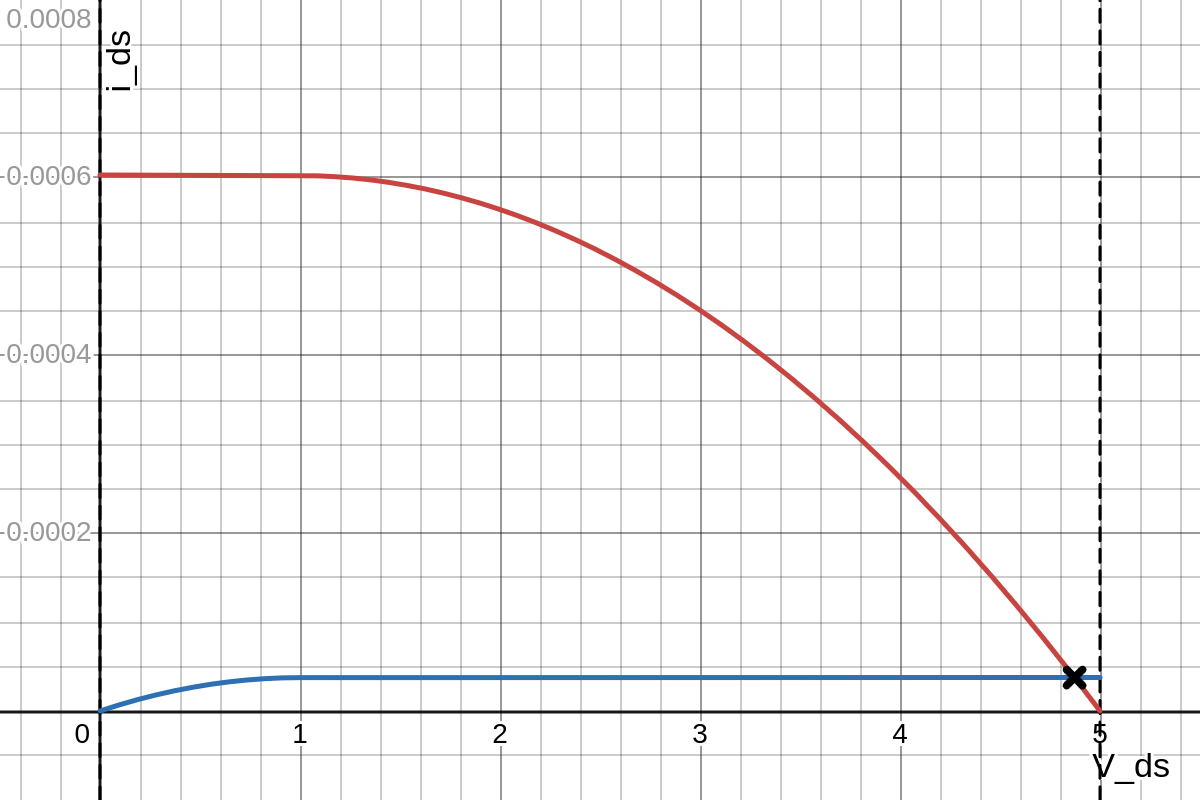
\includegraphics[scale=0.28]{../figures/cmos_inter.png}
\end{center}
da cui è ancora più chiara l'intersezione in corrente che ci interessa (la $V_{DSN}$, o alternativamente $V_{DD} + V_{DSP}$, all'ascissa rappresenta la tensione $V_{out}$ di uscita).

Infine, notiamo che spesso in elettronica la $V_{CC}$ è detta $V_{DD}$ (in quanto alimenta drain di MOSFET e non collettori di BJT).

\subsubsection{Analisi dell'inverter in CMOS complementare}

Iniziamo quindi l'analisi dell'inverter vero e proprio.
Innanzitutto, ricordiamo le equazioni che ci interessano:
\begin{enumerate}
\item I parametri associati all'NMOS sono direttamente legati alla caratteristica di uscita del circuito:
$$
\begin{cases}
V_{DSN} = V_{out} \\
V_{GSN} = V_{in}
\end{cases}
$$
\item Ribaltiamo i parametri associati al PMOS in maniera tale da riportarli al primo quadrante:
$$
\begin{cases}
i_{DP} = -i_{DN} \\
V_{DSP} = V_{DSN} - V_{DD}
\end{cases}
$$
\item Esprimiamo le variabili di controllo (cioè le $V_{GS}$) dell'NMOS e del PMOS in funzione della $V_{in}$:
$$
\begin{cases}
V_{GSN} = V_{in} \\
V_{GSP} = V_{in} - V_{DD}
\end{cases}
$$
\end{enumerate}

Distinguiamo quindi i diversi casi per la $V_{in}$, notando come si ripercuote sulle tensioni fra gate e source dei MOSFET, e quindi l'effetto sulla variabile di uscita:
\begin{enumerate}
\item
\begin{center}
$V_{in} \in [0, V_{TN}]$,
$V_{GSN} \in [0, V_{TN}]$,
$V_{GSP} \in [- V_{DD}, - V_{DD} + V_{TN}]$ 
\end{center}

\begin{center}
	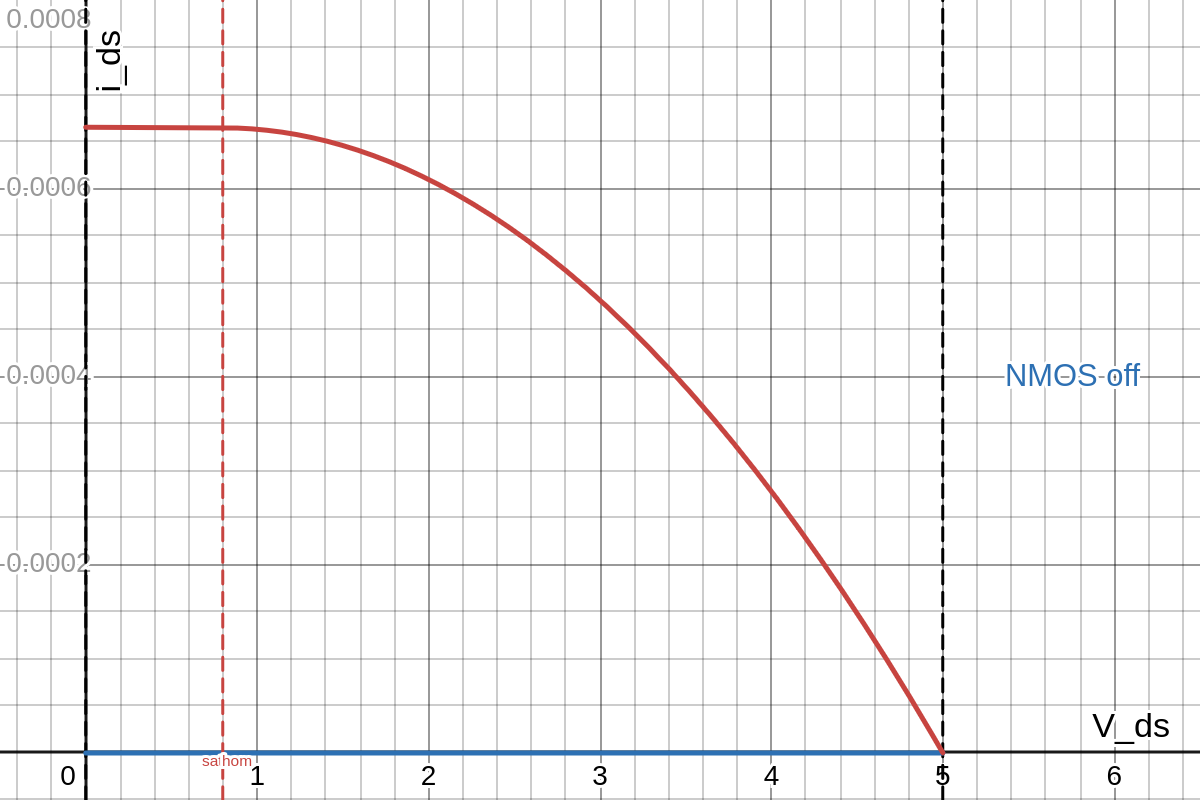
\includegraphics[scale=0.25]{../figures/inv_regions/reg1.png}
\end{center}

\begin{center}
\textsf{NMOS interdetto}, \textsf{PMOS ohmico} \\
\end{center}

In questo caso la caratteristica del PMOS è in conduzione (in quanto $V_{GSP} < 0$), mentre la caratteristica del NMOS è in interdizione (in quanto $V_{GSN} = 0$). Segue che l'unica intersezione possibile è:
$$
\begin{cases}
V_{DSN} = V_{DD} \\ V_{DSP} = 0
\end{cases} \implies
V_{DSN} = V_{DSP} + V_{DD} = 0 + V_{DD}
$$

Questo caso permane fino alla tensione di treshold, cioè finché $V_{in} < V_T$, in quanto l'NMOS non entra ancora in conduzione.

\item 
\begin{center}
$V_{in} \in [V_T, {V_{in}}^*_1]$,
$V_{GSN} \in [V_T, {V_{in}}^*_1]$, 
$V_{GSP} \in [V_T - V_{DD}, {V_{in}}^*_1 - V_{DD}]$ \\
\end{center}

\begin{center}
	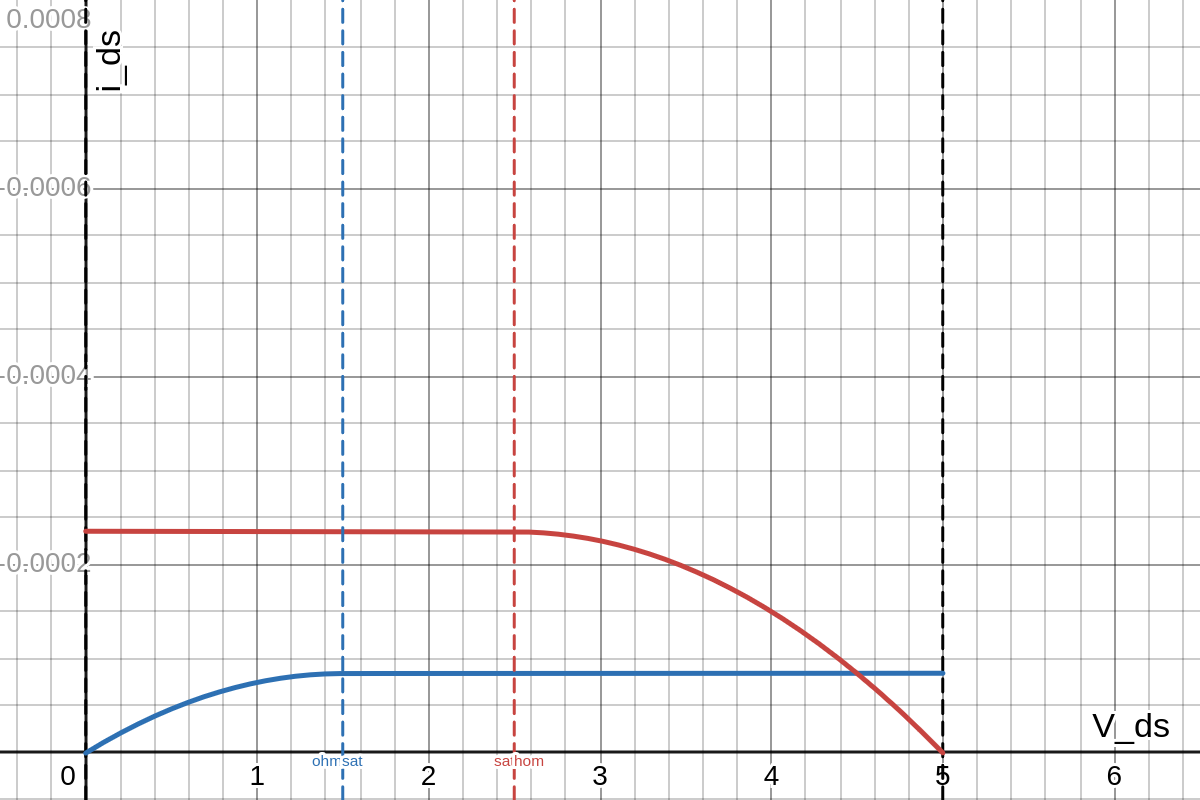
\includegraphics[scale=0.25]{../figures/inv_regions/reg2.png}
\end{center}

\begin{center}
\textsf{NMOS saturo}, \textsf{PMOS ohmico}
\end{center}

In questo caso il PMOS resta in regione triodo, in quanto la tensione al gate è confrontabile con la $V_{T}$. L'NMOS è invece saturo, per cui si ha intersezione in un punto intermedio fra $V_{DD}$ e $0 \, \mathrm{V}$.

Questa situazione permane finché non si entra nella condizione di saturazione del PMOS, cioè finche non è rispettata:
$$
V_{DSP} \geq V_{GSP} - V_{TP}
$$
Ricordando che:
$$
V_{DSP} = V_{DSN} - V_{DD} = V_{out} - V_{DD}, \quad V_{GSP } = V_{in} - V_{DD}
$$
si ha:
$$
V_{out} - V_{DD} \geq V_{in} - V_{DD} - V_{TP} \implies V_{out} \ geq V_{in} - V_{TP}
$$

Chiamiamo la tensione in entrata $V_{in}$ dove questo si verifica ${V_{in}}^*_1$ (per distinguerla, come vedremo da un altro punto dove accade una cosa simile per l'NMOS).

\item 
\begin{center}
$V_{in} \in [{V_{in}}^*_1, {V_{in}}^*_2]$,
$V_{GSN} \in [{V_{in}}^*_1, {V_{in}}^*_2]$,
$V_{GSP} \in [{V_{in}}^*_1 - V_{DD}, {V_{in}}^*_2 - V_{DD}$] \\
\end{center}

\begin{center}
	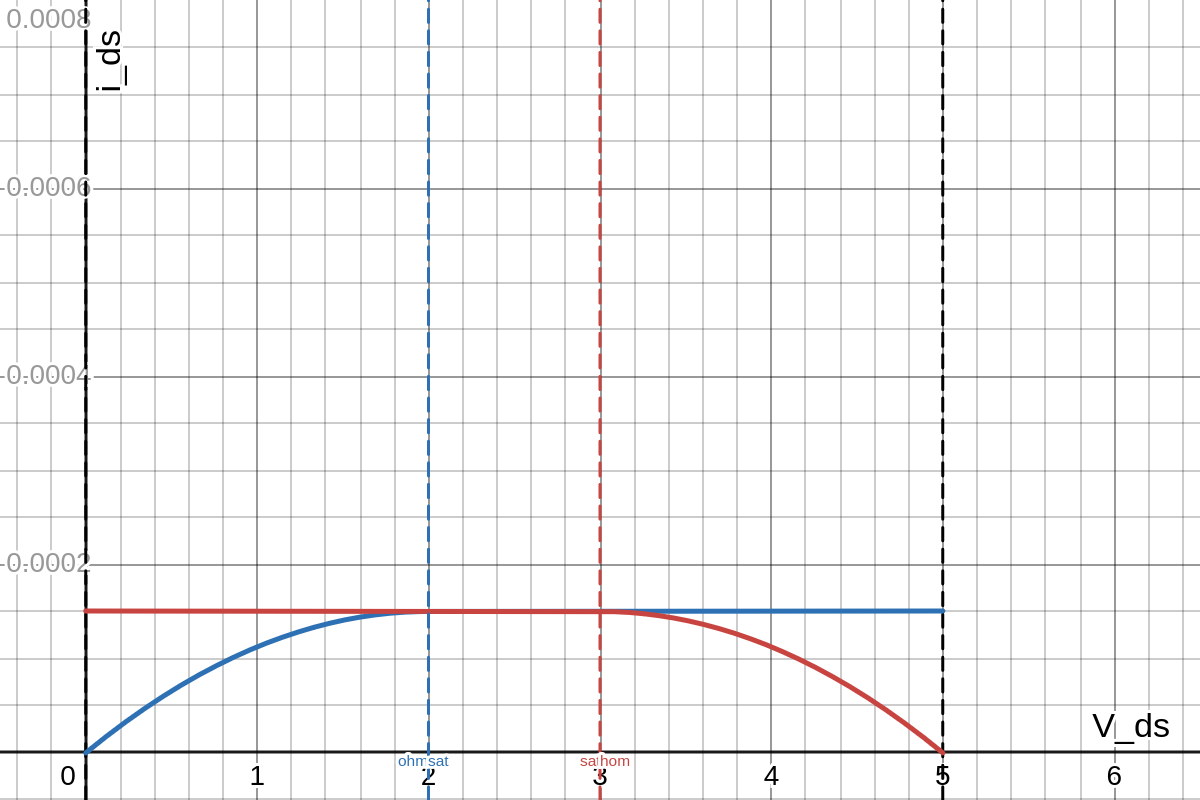
\includegraphics[scale=0.25]{../figures/inv_regions/reg3.png}
\end{center}

\begin{center}
\textsf{NMOS saturo}, \textsf{PMOS saturo}
\end{center}

Questa regione è l'intorno con centro esattamente a metà fra $0 \, \mathrm{V}$ e $V_{DD}$ (assunto $\mu_n = \mu_p$), cioè quello dove il picco raggiunto dalle caratteristiche del PMOS e dell'NMOS è uguale.

Come abbiamo anticipato, questa situazione permane finché il NMOS non esce dalla saturazione, cioè viene meno la condizione:
$$
V_{GSN} \geq V_{GSN} - V_{TN}
$$

Chiamiamo la tensione in entrata $V_{in}$ dove questo si verifica ${V_{in}}^*_2$.

\item 
\begin{center}
$V_{in} \in [{V_{in}}^*_2, V_{DD} + V_{TP}]$,
$V_{GSN} \in [{V_{in}}^*_2, V_{DD} + V_{TP}]$,
$V_{GSP} \in [{V_{in}}^*_2 - V_{DD}, + V_{TP}]$ \\
\end{center}

\begin{center}
	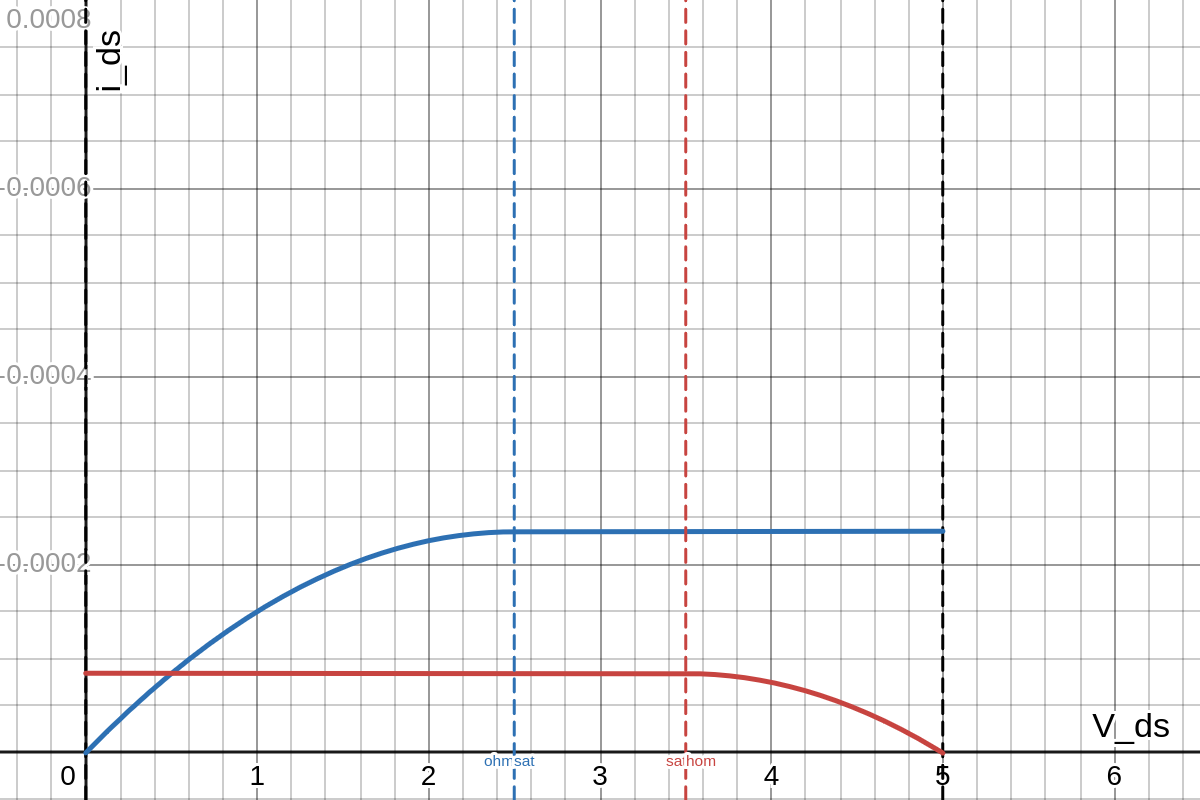
\includegraphics[scale=0.25]{../figures/inv_regions/reg4.png}
\end{center}

\begin{center}
\textsf{NMOS ohmico}, \textsf{PMOS saturo}
\end{center}

In questo caso l'NMOS va in regione triodo, mentre il PMOS resta in saturazione. Questa situazione risulta quindi totalmente duale alla 2, e termina quando viene meno la condizione di conduzione del PMOS. Questo accade quando la $V_{GSP}$ sale sopra $V_{TP}$, o alternativamente quando la $V_{GSN}$ (e quindi $V_{in}$ rispetta):
$$
V_{in} = V_{DD} è V_{TP}
$$
ricordando $V_{TP}$ negativa.

\item 
\begin{center}
$V_{in} \in [V_{DD} + V_{TP}, V_{DD}]$,
$V_{GSN} \in [V_{DD} + V_{TP}, V_{DD}]$,
$V_{GSP} \in [è V_{TP}, 0]$ \\
\end{center}

\begin{center}
	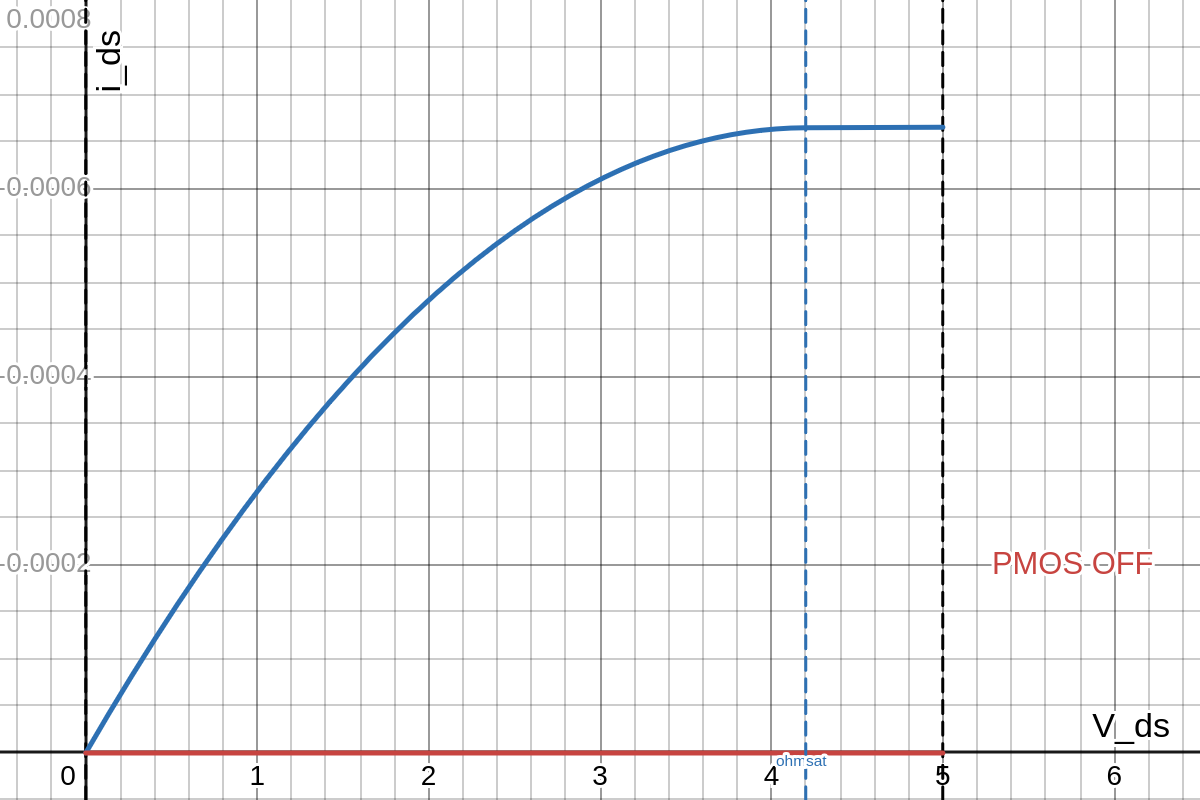
\includegraphics[scale=0.25]{../figures/inv_regions/reg5.png}
\end{center}

\begin{center}
\textsf{NMOS ohmico}, \textsf{PMOS interdetto}
\end{center}

Questa è la situazione in cui ci troviamo quandoil PMOS smette di condurre.
Segue che si ha l'intersezione in $V_{out} = 0 \, \mathrm{V}$, in quanto:
$$
\begin{cases}
V_{DSN} = 0 \, \mathrm{V} \\ V_{DSP} = -V_{DD}
\end{cases} \implies
V_{DSN} = V_{DSP} + V_{DD} = - V_{DD} + V_{DD} = 0 \, \mathrm{V}
$$

\end{enumerate}

\par\smallskip

Abbiamo quindi individuato 5 regioni per descrivere il comportamento di questo circuito, controllando le conduzioni di conduzione e di saturazione di entrambi i MOSFET. Riguardo alle disuguaglianze che delimitano tali regioni abbiamo che che:

\par\medskip

\noindent
\begin{minipage}[t]{0.48\textwidth}
\textbf{\textsf{NMOS}}
\begin{itemize}
	\item \textbf{Conduzione}: $V_{GSN} = V_{in} \geq V_{TN}$
		$$
		\implies V_{in} \geq V_{TN}
		$$
	\item \textbf{Saturazione}: $V_{DSN} \geq V_{GSN} - V_{TN}$
		$$
		\implies V_{out} \geq V_{in} - V_{TN}
		$$
\end{itemize}

\end{minipage}\hfill
\begin{minipage}[t]{0.48\textwidth}
\textbf{\textsf{PMOS}}
\begin{itemize}
	\item \textbf{Conduzione}: $V_{GSP} \leq V_{TP}$
		$$
		\implies V_{in} \leq V_{DD} + V_{TP}
		$$
	\item \textbf{Saturazione}: $V_{DSP} \geq V_{GSP} - V_{TP}$
		$$
		\implies V_{out} \geq V_{in} - V_{TP}
		$$
\end{itemize}
\end{minipage}

\par\bigskip

\noindent
\textbf{\textsf{Tracciamento della VTC}}

\noindent
Dopo aver ricavato con esattezza quali sono le regioni che possiamo individuare per l'inverter in tecnologia CMOS, applichiamo le caratteristiche di uscita del PMOS e il NMOS per impostare i sistemi ad ogni regione. Quindi, risolviamo per ricavare un espressione della $V_{out}$ in funzione della $V_{in}$ in ogni regione. In altre parole, andiamo a calcolare analitcamente, e successivamente tracciare, la \textbf{VTC} (\textit{Voltage Transfer Characteristic}).  

I calcoli che seguono sono stati verificati tracciando la VTC nel Desmos reperibile in \url{https://www.desmos.com/calculator/917i39rpoz}.

Iniziamo quindi dall'impostare le caratteristiche dell'NMOS e del PMOS in funzione di $V_{in}$ e $V_{out}$. Per fare ciò, ricordiamo, che i parametri dell'NMOS si riflettono direttamente nei parametri dell'inverter: 
$$
\begin{cases}
V_{DSN} = V_{out} \\
V_{GSN} = V_{in}
\end{cases}
$$
mentre per il ribaltamento della caratteristica del PMOS si era imposto:
$$
\begin{cases}
i_{DP} = -i_{DN} \\
V_{DSP} = V_{DSN} - V_{DD} = V_{out} - V_{DD}
\end{cases}
$$
dove l'uguaglianza era in $i_{DP} = -i_{DN}$. Per risparmiarci un segno meno, prendiamo equivalentemente:
$$
i_{DN} = i_{SP}
$$
cioè la corrente al PMOS uscente dal source anziché dal drain.

Da queste considerazioni segue che le caratteristiche sono, trascurando il termine $K$ (che assumiamo uguale per MOSFET PMOS e NMOS, e cancellerebbe nei sistemi):
\begin{itemize}
\item Per il NMOS:
$$
\begin{cases}
	i_{DN}=\left(\left(V_{in}-V_{TN}\right)V_{out}-\frac{V_{out}^{2}}{2}\right) & \text{(triodo)} \\
	i_{DN}=\frac{1}{2}\left(V_{in}-V_{TN}\right)^{2} & \text{(saturazione)} \\
	i_{DN}=0 & \text{(interdizione)}
\end{cases}
$$
\item Per il PMOS:
$$
\begin{cases}
	i_{SP}=\left(\left(V_{GSP}-V_{TP}\right)\left(V_{out}-V_{DD}\right)-\frac{V_{DSP}^{2}}{2}\right) & \text{(triodo)}\\
	i_{SP}=\frac{1}{2}\left(V_{DSP}-V_{TP}\right)^{2} & \text{(saturazione)} \\
	i_{SP}=0 & \text{(interdizione)}
\end{cases}
$$
dove le equazioni sono le stesse viste in 16.0.3, con la differenza che la variabile per $V_{SD}$ è $V_{DSP}$ (cioè ha segno invertito nel primo termine della zona triodo). 
Imponendo il ribaltamento, e imponendo per la tensione al gate $V_{GSN} = V_{in} - V_{DD}$ (un altra delle equazioni cardine, che non abbiamo riportato in questa sezione) si ricava allora:
$$
\begin{cases}
i_{SP}=\left(\left(V_{in}-V_{DD}-V_{TP}\right)\left(V_{out}-V_{DD}\right)-\frac{\left(V_{out}-V_{DD}\right)^{2}}{2}\right) & \text{(triodo)}\\
i_{SP}=\frac{1}{2}\left(V_{in}-V_{DD}-V_{TP}\right)^{2} & \text{(saturazione)} \\
i_{SP}=0 & \text{(interdizione)}
\end{cases}
$$
\end{itemize}

A questo punto impostiamo i sistemi per ogni regione:
\begin{enumerate}
\item
\begin{center}
$V_{in} \in [0, V_{TN}]$,
$V_{GSN} \in [0, V_{TN}]$,
$V_{GSP} \in [- V_{DD}, - V_{DD} + V_{TN}]$ 
\end{center}

% regione 1
In questa situazione l'\textbf{NMOS} è \textit{interdetto} e il \textbf{PMOS} in \textit{triodo}, per cui il sistema si pone come
$$
\begin{cases}
i_{DN}=0 & \text{(NMOS in interdizione)} \\
i_{SP}=\left(\left(V_{GSP}-V_{TP}\right)\left(V_{out}-V_{DD}\right)-\frac{V_{DSP}^{2}}{2}\right) & \text{(PMOS in triodo)}\\
\end{cases}
$$

Senza particolari sorprese, la soluzione è costante al $V_{DD}$, in quanto la $i_{DN}$ fissa il punto in cui campioniamo la $V_{DSN}$:
$$
r_{1}\left(V_{in}\right)=V_{DD}\ \left\{0<V_{in}<V_{TN}\right\}
$$

\item 
\begin{center}
$V_{in} \in [V_T, {V_{in}}^*_1]$,
$V_{GSN} \in [V_T, {V_{in}}^*_1]$, 
$V_{GSP} \in [V_T - V_{DD}, {V_{in}}^*_1 - V_{DD}]$ \\
\end{center}

% regione 2
In questa situazione l'\textbf{NMOS} è in \textit{saturazione} e il \textbf{PMOS} in \textit{triodo}, per cui il sistema si pone come
$$
\begin{cases}
i_{DN}=\frac{1}{2}\left(V_{in}-V_{TN}\right)^{2} & \text{(NMOS in saturazione)} \\
i_{SP}=\left(\left(V_{GSP}-V_{TP}\right)\left(V_{out}-V_{DD}\right)-\frac{V_{DSP}^{2}}{2}\right) & \text{(PMOS in triodo)}\\
\end{cases}
$$

Si risparmia la soluzione del sistema, ma si ha che questo dà vita a una quadratica che risolve in:
$$
r_{2}\left(V_{in}\right)=\left(V_{in}-V_{TP}\right)+\sqrt{\left(V_{in}-V_{DD}-V_{TP}\right)^{2}-\left(V_{in}-V_{TN}\right)^{2}}\left\{V_{TN}<V_{in}<{V_{in}}^*_1\right\}
$$

Diamo quindi il valore della ${V_{in}}^*_1$. Questo sarà dato imponendo la caratteristica della seconda regione uguale alla barriera della condizione:
$$
V_{out} = V_{in} - V_{TP}
$$
per la saturazione del PMOS, da cui:
$$
{V_{in}}^*_1=\frac{V_{TN}+V_{DD}+V_{TP}}{2}
$$

\item 
\begin{center}
$V_{in} \in [{V_{in}}^*_1, {V_{in}}^*_2]$,
$V_{GSN} \in [{V_{in}}^*_1, {V_{in}}^*_2]$,
$V_{GSP} \in [{V_{in}}^*_1 - V_{DD}, {V_{in}}^*_2 - V_{DD}$] \\
\end{center}

% regione 3
In questa situazione l'\textbf{NMOS} è in \textit{saturazione} e il \textbf{PMOS} in \textit{saturazione}, per cui il sistema si pone come
$$
\begin{cases}
i_{DN}=\frac{1}{2}\left(V_{in}-V_{TN}\right)^{2} & \text{(NMOS in saturazione)} \\
i_{SP}=\frac{1}{2}\left(V_{in}-V_{DD}-V_{TP}\right)^{2} & \text{(PMOS in saturazione)} \\
\end{cases}
$$

Questo sistema è il più semplice da risolvere (e sicuramente il più interessante per quanto riguarda la caratteristica dell'inverter). Abbiamo infatti che in questa regione la VTC è completamente verticale (faremo delle considerazioni in seguito riguardo a ciò). 

Il valore della $V_{in}$ nella retta verticale individuatà sarà:
$$
r_{3}=\frac{V_{DD}+V_{TP}+V_{TN}}{2}\ \left\{V_{out2}<y<V_{out1}\right\}
$$
dove i parameteri $V_{out2}$ e $V_{out1}$ si calcolano a partire dall'equazione della regione 2 (già vista) e della regione 4 (che vedremo fra poco), valutate rispettivamente nei punti estremi ${V_{in}}^*_2$ e ${V_{in}}^*_1$.

\item 
\begin{center}
$V_{in} \in [{V_{in}}^*_2, V_{DD} + V_{TP}]$,
$V_{GSN} \in [{V_{in}}^*_2, V_{DD} + V_{TP}]$,
$V_{GSP} \in [{V_{in}}^*_2 - V_{DD}, + V_{TP}]$ \\
\end{center}

\begin{center}
\textsf{NMOS ohmico}, \textsf{PMOS saturo}
\end{center}

% regione 4
In questa situazione l'\textbf{NMOS} è in \textit{triodo} e il \textbf{PMOS} in \textit{saturazione}, per cui il sistema si pone come
$$
\begin{cases}
i_{DN}=\left(\left(V_{in}-V_{TN}\right)V_{out}-\frac{V_{out}^{2}}{2}\right) & \text{(NMOS in triodo)} \\
i_{SP}=\frac{1}{2}\left(V_{in}-V_{DD}-V_{TP}\right)^{2} & \text{(PMOS in saturazione)} \\
\end{cases}
$$

Questo caso è esattamente il duale della regione 2, ma con i transistor scambiati di ruolo. Anche la soluzione del sistema ha soluzione simile:
$$
r_{4}\left(V_{in}\right)=\left(V_{in}-V_{TN}\right)-\sqrt{\left(V_{in}-V_{TN}\right)^{2}-\left(V_{in}-V_{DD}-V_{TP}\right)^{2}}\ \left\{V_{in2}<V_{in}<V_{DD}+V_{TP}\right\}
$$

Anche qui possiamo dare il valore della ${V_{in}}^*_2$. Questo sarà dato imponendo la caratteristica della quarta regione uguale alla barriera della condizione:
$$
V_{out} = V_{in} - V_{TN}
$$
per la saturazione dell'NMOS, per cui:
$$
{V_{in}}^*_2=\frac{V_{TN}+V_{DD}+V_{TP}}{2}
$$

Vediamo quindi che ${V_{in}}^*_1 = {V_{in}}^*_2$. Questa non è altro che un'affermazione alternativa del fatto che la VTC è verticale nella regione di saturazione sia del PMOS che dell'NMOS (cioè la regione 3);

\item 
\begin{center}
$V_{in} \in [V_{DD} + V_{TP}, V_{DD}]$,
$V_{GSN} \in [V_{DD} + V_{TP}, V_{DD}]$,
$V_{GSP} \in [è V_{TP}, 0]$ \\
\end{center}

% regione 5
In questa situazione l'\textbf{NMOS} è in \textit{triodo} e il \textbf{PMOS} \textit{interdetto}, per cui il sistema si pone come
$$
\begin{cases}
i_{DN}=\left(\left(V_{in}-V_{TN}\right)V_{out}-\frac{V_{out}^{2}}{2}\right) & \text{(NMOS in triodo)} \\
i_{SP}=0 & \text{(PMOS in interdizione)} \\
\end{cases}
$$

Questo caso è esattamente il duale della regione 1, ma con i transistor scambiati di ruolo. Anche la soluzione del sistema è banale, in quanto la $i_{SP}$ fissa il punto in cui campioniamo la $V_{DSP}$:
$$
r_{5}\left(V_{in}\right)=0\ \left\{V_{DD}+V_{TP}<V_{in}<V_{DD}\right\}
$$
\end{enumerate}

Possiamo quindi tracciare le curve trovate per tracciare l'intera curva caratteristica della VTC:
\begin{center}
	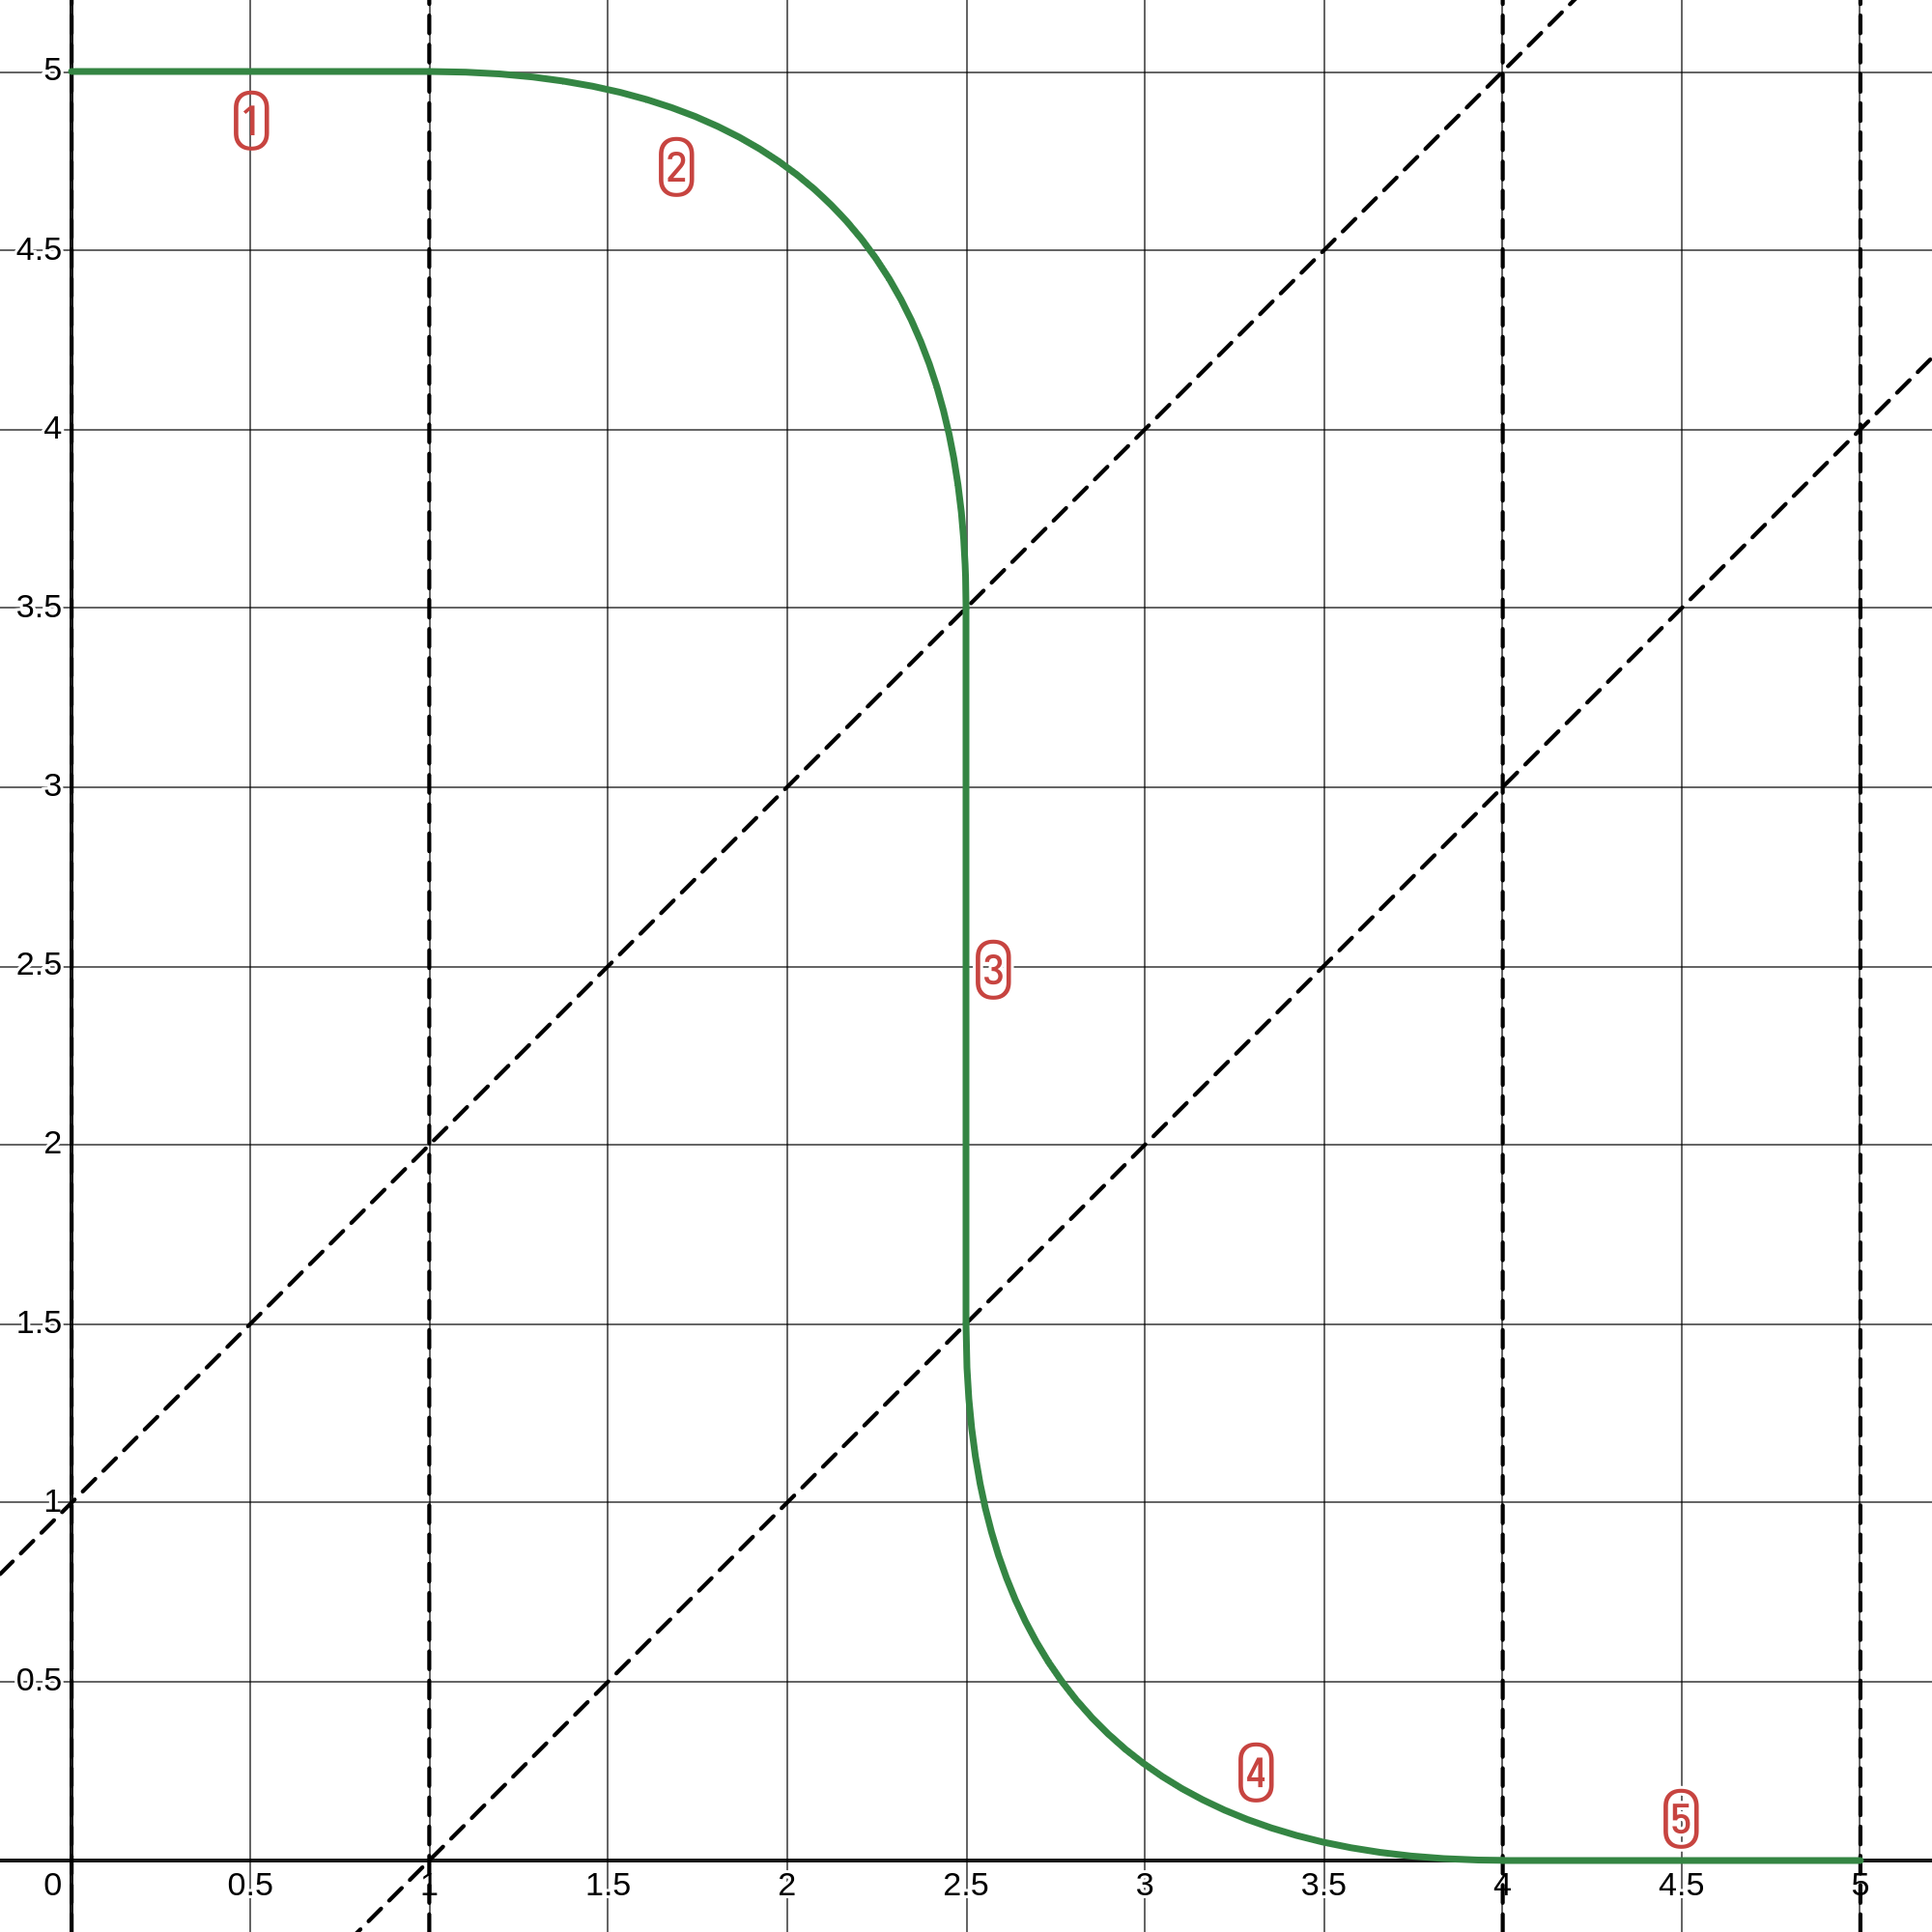
\includegraphics[scale=0.2]{../figures/inv_vtc.png}
\end{center}
dove sono state evidenziate tutte le regioni che vengono attraversate. Le righe verticali rappresentano rispettivamente le barriere, da sinistra verso destra:
$$
V_{in} = V_{TN}, \quad V_{in} = V_{DD} - V_{TP}
$$
mentre le righe diagonali rappresentano, sempre da sinistra verso destra:
$$
V_{out} = V_{in} - V_{TP}, \quad V_{out} = V_{in} - V_{TN}
$$
da cui notiamo ad esempio che si incontra la saturazione del PMOS prima della desaturazione dell'NMOS (transizioni fra 2 e 3, e fra 3 e 2). 

\par\smallskip

\noindent
\textbf{\textsf{Verticalità della regione 3}}

\noindent
Come anticipato, facciamo delle considerazioni aggiuntive sulla regione 3. Questa ha la particolarità, nel caso ideale, di essere completamente verticale. Chiaramente non sarà questo il caso in un inverter reale, per via del fatto che si ha l'effetto modulazione di campo che introduce una piccola resistenza in serie al modello del MOSFET in conduzione.

Anche senza considerare l'effetto modulazione di campo, però, abbiamo delle considerazioni interessanti se trascuriamo la semplificazione che abbiamo fatto prima, cioè di dire:
$$
K_n = K_p, \quad \left( \mu_n C_{ox} \frac{W}{L} = \mu_p C_{ox} \frac{W}{L} \right)
$$

Vediamo l'effetto che questo ha nella regione 3. Il sistema si presenterà come:
$$
\begin{cases}
	K_N (V_{GSN} - V_{TN})^2 = K_P (V_{GSP} - V_{TP})^2 \\
	V_{GSN} = V_{in} \\
	V_{GSP} = V_{in} - V_{DD}
\end{cases}
\implies
K_N (V_{in} - V_{TN})^2 = K_P (V_{in} - V_{DD} - V_{TP})^2
$$
che prendendo la radice ed evidenziando $V_{in}$ dà:
$$
V_{in} = \frac{\sqrt{K_p} (V_{DD} + V_{TP}) + \sqrt{K_n} V_{TN} }{\sqrt{K_n} + \sqrt{K_p}}
$$
questa decade nella forma che avevamo visto prima, nel caso $K_n = K_p$:
$$
K_n = K_p \implies V_{in} = \frac{V_{DD} + V_{TP} + V_{TN}}{2}
$$


La cosa importante è che variare $K_n$ e $K_p$ varia l'equilibrio della VTC, cioè il punto in cui questa diventa approssimativamente verticale. Questo è chiaro notando che se $K_n > K_p$, il punto verticale viene "trascinato" verso sinistra nel grafico, cioè verso la regione vicina a $V_{in} = 0 \, \mathrm{V}$. Viceversa, se si aumenta la $K_p$ fino a $K_p > K_n$ accade il contrario.

Proprio per questo motivo nella maggior parte dei dispositivi reali si cerca di mantenere $K_n$ e $K_p$ costanti. Visto che questi sono effettivamente parametri sotto nostro controllo (in base alla larghezza e la lunghezza del canale del MOSFET), almeno nei circuiti integrati, mentre le vere costanti fisiche sono $\mu_n$ e $\mu_p$, basta verificare:
$$
\frac{\mu_n}{\mu_p} = \frac{ \left( \frac{W}{L} \right)_P }{ \left( \frac{W}{L} \right)_N }
$$
che è una delle equazioni più importanti della microelettronica.


\end{document}

